\documentclass[10pt,a4paper]{article}
\usepackage{nexusS5}
\setnexusheader{Entrée en Seconde générale et technologique — Stage de pré-rentrée}{Séance 5/5 — Noa MANIACI}
\begin{document}
\nexuscover{SÉANCE 5 --- RÉINVESTIR, CONSOLIDER, PRÉPARER LA RENTRÉE}{Livret de travail}{Noa MANIACI}{Installer les équations et les évolutions}{Entrée en Seconde générale et technologique --- Mathématiques --- 1\,h\,15 de travail, puis 45 minutes d'évaluation dans un document séparé}
\begin{goalbox}
\textbf{Objectif personnel de cette séance.} Écrire la relation avant le calcul et effectuer un contrôle de vraisemblance — conseil du dossier — en installant d'abord l'équation produit nul puis les évolutions successives.
\par\medskip
\textbf{Ce livret couvre uniquement les 75 premières minutes.} L'évaluation finale est remise ensuite, dans un document distinct.
\end{goalbox}
\begin{methodbox}
\textbf{Le fil des cinq séances}
\begin{itemize}[leftmargin=13mm,labelsep=3mm,itemsep=1.5pt]
\item[\textbf{\color{Navy}S1}] Réparer le moteur de calcul (priorités, fractions, puissances) ;
\item[\textbf{\color{Navy}S2}] Construire l'algèbre du lycée (développement, factorisation, équations) ;
\item[\textbf{\color{Navy}S3}] Modéliser une situation (pourcentages, fonctions) ;
\item[\textbf{\color{Navy}S4}] Choisir le bon théorème (Pythagore, Thalès, trigonométrie) ;
\item[\textbf{\color{Navy}S5}] aujourd'hui : réactiver, consolider deux axes personnels, faire le pont vers la Seconde, puis mesurer.
\end{itemize}
\end{methodbox}
\sectiontitle{Feuille de route des 75 minutes}
\rowcolors{2}{SoftBlue}{white}
\par\noindent\begin{tabularx}{\linewidth}{>{\bfseries}p{20mm} X X}
\rowcolor{Navy}\color{white}Temps & \color{white}Travail & \color{white}Preuve attendue \\
0--10 min & Réactiver les automatismes de calcul et d'algèbre qui conditionnent les premières semaines de Seconde. & Cinq réponses écrites et le contrôle utilisé. \\
10--35 min & Équation produit nul & Trois réussites autonomes sur l'axe prioritaire. \\
35--55 min & Coefficient multiplicateur et évolutions successives & Deux réussites autonomes sur le second axe. \\
55--70 min & De la Troisième à la Seconde : intervalles et langage des fonctions & Une production reliant un acquis de Troisième à un attendu de Seconde. \\
70--75 min & Cadrage méthodologique, sans aucune information sur le contenu de l'évaluation. & Deux engagements écrits avant l'évaluation. \\
\end{tabularx}
\begin{graybox}\small\textbf{Règle de la séance.} J'écris ma réponse \emph{et} le contrôle qui la rend défendable. Une réponse sans contrôle reste une hypothèse. La ligne « Certitude » se remplit \emph{avant} toute vérification.\end{graybox}
\par\vspace{2mm}
\phasehead{Phase 1 --- Réactivation}{0--10 min}{Réactiver les automatismes de calcul et d'algèbre qui conditionnent les premières semaines de Seconde.}
Sept minutes seules, sans carte de rappel, puis trois minutes de mise en commun. Écrire la réponse \emph{et} le contrôle utilisé.
\begin{enumerate}
\item Calculer $-5 + 3\times(-4) - (-2)$.
\shortlines{2}
\item Calculer $\dfrac{5}{6}\div\dfrac{10}{9}$ et simplifier.
\shortlines{2}
\item Développer et réduire $(x-3)(x+7)$.
\shortlines{2}
\item Résoudre $(3x-6)(x+4)=0$.
\shortlines{2}
\item Écrire $0{,}00058$ en notation scientifique.
\shortlines{2}
\end{enumerate}
\certline
\aideline
\needspace{62mm}\par\vspace{3mm}
\phasehead{Phase 2 --- Consolidation, axe prioritaire}{10--35 min}{Équation produit nul}
\begin{methodbox}
\textbf{Une propriété, pas une manipulation.} Un produit de facteurs est nul \textbf{si et seulement si}
l'un au moins des facteurs est nul. Une équation sous forme factorisée ne doit donc \textbf{jamais} être développée.
\textbf{Contrôle :} une équation produit à deux facteurs distincts possède en général deux solutions.
\end{methodbox}
\begin{graybox}
\textbf{Exemple guidé.} Résoudre $(2x - 6)(x + 5) = 0$.
\begin{enumerate}
\item Propriété : le produit est nul, donc $2x - 6 = 0$ ou $x + 5 = 0$.
\item Première équation : $2x = 6$, donc $x = 3$.
\item Seconde équation : $x = -5$.
\item Contrôler $x = 3$ : $(0)\times 8 = 0$. Contrôler $x = -5$ : $(-16)\times 0 = 0$.
\end{enumerate}
\end{graybox}
\subsectiontitle{À toi}
\begin{enumerate}
\needspace{18mm}
\item Résoudre $(x - 7)(x + 2) = 0$.
\worklines{3}
\needspace{18mm}
\item Résoudre $(3x + 9)(2x - 5) = 0$.
\worklines{3}
\needspace{18mm}
\item Résoudre $x(x - 4) = 0$.
\worklines{3}
\needspace{18mm}
\item Factoriser $x^2 - 5x$, puis résoudre $x^2 - 5x = 0$.
\worklines{4}
\needspace{18mm}
\item Vérifier que $-4$ est solution de $(x + 4)(3x - 1) = 0$, puis donner l'autre solution.
\worklines{3}
\needspace{18mm}
\item Un élève résout $(3x + 5)(x - 2) = 0$ en développant d'abord. Expliquer pourquoi la forme factorisée est préférable et ce qu'il risque de perdre.
\worklines{4}
\end{enumerate}
\begin{successbox}\textbf{Critère de réussite de cette phase :} trois équations produit résolues consécutivement avec les deux solutions et la propriété citée.\end{successbox}
\certline
\needspace{62mm}\par\vspace{3mm}
\phasehead{Phase 3 --- Consolidation, second axe}{35--55 min}{Coefficient multiplicateur et évolutions successives}
\begin{methodbox}
\textbf{Un pourcentage se traduit par un coefficient.} Une hausse de $t\,\%$ correspond au coefficient
$1 + \frac{t}{100}$, une baisse de $t\,\%$ au coefficient $1 - \frac{t}{100}$.
\par\smallskip
\textbf{Deux évolutions successives se multiplient, elles ne s'additionnent jamais.}
\textbf{Contrôle :} un coefficient global supérieur à $1$ signifie une hausse globale, inférieur à $1$ une baisse.
\end{methodbox}
\subsectiontitle{À toi}
\begin{enumerate}
\needspace{18mm}
\item Un prix de $340$ TND augmente de $15\,\%$. Calculer le nouveau prix.
\worklines{2}
\needspace{18mm}
\item Un prix de $340$ TND baisse de $15\,\%$. Calculer le nouveau prix.
\worklines{2}
\needspace{18mm}
\item Donner le coefficient multiplicateur d'une hausse de $8\,\%$, puis celui d'une baisse de $8\,\%$.
\worklines{2}
\needspace{18mm}
\item Un prix augmente de $10\,\%$ puis de $30\,\%$. Le coefficient global vaut-il $1{,}40$ ? Justifier par le calcul.
\worklines{4}
\end{enumerate}
\begin{successbox}\textbf{Critère de réussite de cette phase :} trois situations d'évolution traitées consécutivement par coefficient multiplicateur, dont une composée, avec conclusion argumentée.\end{successbox}
\certline
\needspace{62mm}\par\vspace{3mm}
\phasehead{Phase 4 --- Réinvestissement}{55--70 min}{Découverte guidée : construire, à partir du calcul et des équations déjà travaillés, deux notations nouvelles de Seconde — l'intervalle et le langage des fonctions.}

\begin{methodbox}
\textbf{Ce qui change en Seconde.} Deux outils \textbf{nouveaux} apparaissent dès les premières semaines :
l'\textbf{intervalle}, qui remplace les phrases du type « $x$ est compris entre... », et le \textbf{langage
des fonctions}, qui donne un statut nouveau aux expressions littérales déjà manipulées.
\par\smallskip
\textbf{Ce qui est réinvesti} : le calcul numérique, la substitution et l'équation produit nul, travaillés
en séances 1 et 2. \textbf{Ce qui est nouveau} : la notation en intervalle et le vocabulaire fonctionnel.
Les deux blocs ci-dessous sont donc une \textbf{découverte guidée}, non un réemploi.
\end{methodbox}
\begin{warningbox}\small
\textbf{Cette phase introduit des notions de l'année à venir.} Ce que tu produis ici ne sera donc
\emph{pas} comparé à ton positionnement de début de stage : il ne s'agit pas de mesurer un progrès,
mais de préparer les premières séances de septembre.
\end{warningbox}


\subsectiontitle{A. De l'inégalité à l'intervalle — 6 min}
\par\noindent\begin{tabularx}{\linewidth}{>{\bfseries}p{40mm} X X}
\toprule
Phrase & Inégalité & Intervalle \\
\midrule
$x$ est strictement supérieur à $2$ & & \\
$x$ est inférieur ou égal à $5$ & & \\
$x$ est compris entre $-2$ (inclus) et $3$ (exclu) & & \\
$x$ est un nombre quelconque & & \\
\bottomrule
\end{tabularx}
\par\vspace{1.5mm}
Placer ensuite sur l'axe l'ensemble $[-2\,;3[$ en marquant clairement les bornes ouvertes et fermées.
\begin{center}
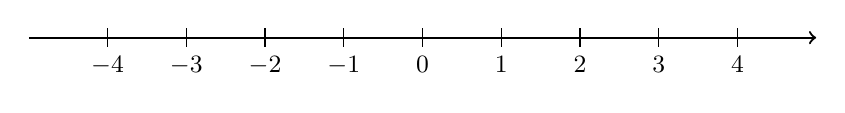
\begin{tikzpicture}[x=1cm]
\draw[->,thick] (-5,0) -- (5,0);
\foreach \x in {-4,-3,-2,-1,0,1,2,3,4}{\draw (\x,0.12) -- (\x,-0.12) node[below]{\small $\x$};}
\end{tikzpicture}
\end{center}

\subsectiontitle{B. D'un programme de calcul à une fonction — 9 min}
Programme : « choisir un nombre, l'élever au carré, puis retrancher le triple du nombre ».
\begin{enumerate}
\item Écrire l'expression obtenue en partant de $x$ ; on la note $f(x)$. \rule{50mm}{0.32pt}
\item Calculer $f(4)$ et $f(-2)$ en écrivant la substitution complète, parenthèses comprises.
\shortlines{2}
\item Compléter le tableau de valeurs.
\end{enumerate}
\par\noindent\begin{tabularx}{\linewidth}{|>{\bfseries}p{18mm}|X|X|X|X|X|X|}
\hline
$x$ & $-2$ & $-1$ & $0$ & $1$ & $3$ & $4$ \\ \hline
$f(x)$ & & & & & & \\ \hline
\end{tabularx}
\begin{enumerate}\setcounter{enumi}{3}
\item Déterminer un antécédent de $0$ par $f$ en écrivant une équation produit nul.
\worklines{2}
\item Vrai ou faux : « le point de coordonnées $(3\,;0)$ appartient à la courbe de $f$ ». Justifier par un calcul.
\shortlines{1}
\end{enumerate}

\begin{successbox}
\textbf{Preuve attendue :} la substitution d'un nombre négatif est écrite avec des parenthèses, et l'antécédent
est obtenu par une équation, non par lecture approximative.
\end{successbox}

\needspace{62mm}\par\vspace{3mm}
\phasehead{Phase 5 --- Avant l'évaluation}{70--75 min}{Cadrage méthodologique. Aucun contenu de l'évaluation n'est annoncé.}

\begin{methodbox}
\textbf{Cinq règles, et rien d'autre.} Ce cadrage ne porte sur aucun contenu de l'évaluation.
\begin{enumerate}
\item \textbf{Gérer le temps.} Trois parties : environ 10 min, 20 min et 15 min. Un regard sur l'horloge à la fin de chaque partie suffit.
\item \textbf{Justifier.} Écrire la relation, la propriété ou la règle avant le calcul. Un résultat seul ne montre pas ce que tu sais.
\item \textbf{Contrôler.} Avant de passer à la suite : ordre de grandeur, substitution, unité, ou vérification par une seconde voie.
\item \textbf{Lire jusqu'au bout.} Souligner la question réellement posée et les données effectivement fournies.
\item \textbf{Passer et revenir.} Une question laissée de côté puis reprise vaut mieux qu'une réponse écrite au hasard.
\end{enumerate}
\end{methodbox}

\begin{graybox}
\textbf{La certitude.} Elle est demandée à trois moments seulement, comme au test de positionnement de début de stage :
\conf\ . Elle n'entre pas dans la note. Elle sert à distinguer ce que tu sais de ce que tu crois savoir.
\end{graybox}

\subsectiontitle{Mon engagement d'avant-évaluation}
\par\vspace{1mm}
\noindent\textbf{Le contrôle que j'écrirai systématiquement :}\ \rule{\dimexpr\linewidth-76mm\relax}{0.32pt}
\par\vspace{3mm}
\noindent\textbf{La question que je traiterai en dernier :}\ \rule{\dimexpr\linewidth-68mm\relax}{0.32pt}
\par\vspace{1mm}

\begin{warningbox}\textbf{Fin du livret de travail.} L'évaluation finale est un document séparé, remis par l'enseignant à l'issue de ces 75 minutes.\end{warningbox}
\end{document}
